
\documentclass{article}

\usepackage{pttyr_descriptions}


\begin{document}

\setlist{nolistsep}
\nointerlineskip
\par\noindent
\setlength{\parindent}{0pt}


\section*{Convolutional Layers}
\subsection*{\ttt{torch.nn.Conv2d}}
\prepostc{torch.nn.Conv2d(in\_channels, out\_channels, kernel\_size, stride=1,
padding=0, dilation=1, groups=1, other\_params..)(x)}{
  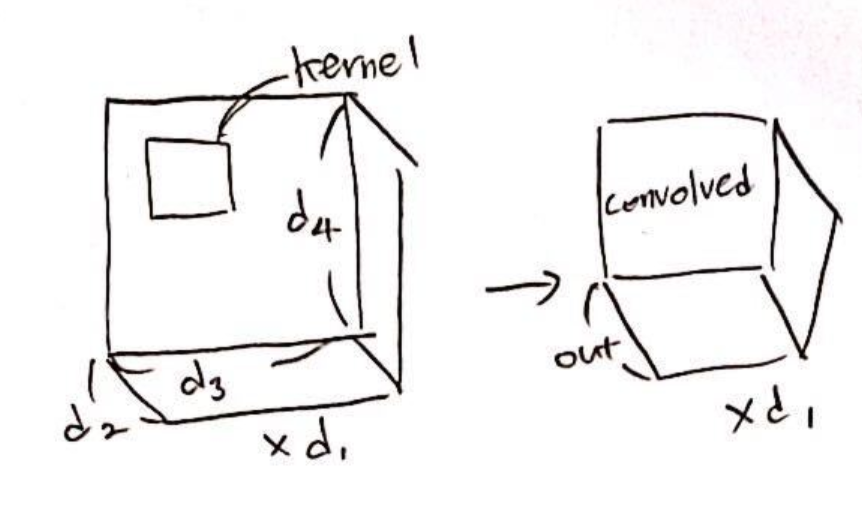
\includegraphics[height=12em]{resources/conv2d.png}
}{
  \begin{itemizec}
    \item $|x| = (d_1, d_2, d_3, d_4)$\bigspace ($rank = 4$)
    \item $d_2 = in\_channels$
    \item $d_3 + 2 \x padding[0] - dilation[0] \x (kernel\_size[0] - 1) - 1 \geq
    0$
    \item $d_4 + 2 \x padding[1] - dilation[1] \x (kernel\_size[1] - 1) - 1 \geq
    0$
    \item $groups | in\_channels$ and $groups | out\_channels$
  \end{itemizec}
}{
  \begin{itemizec}
    \item $|y| = (d_1, out\_channels, h, w)$ where.. refers to the proof tree.
  \end{itemizec}
}{
  \begin{itemizec}
    \item Convolution layer입니다. 선배님의 자료를 \ttt{pytorch}의 사용에 맞게
    풀어 쓴 것입니다.
    \item $kernel\_size$, $stride$와 같은 옵션은 튜플로 구성될 수도 있습니다.
    (가로 세로에 대한 필터크기가 서로 다르도록) 이 경우를 위하여 proof 트리에서
    $kernel\_size[0], [1]$과 같은 표기를 사용하였습니다. 튜플이 아니라 스칼라
    입력인 경우, $kernel\_size[0], [1]$은 모두 $kernel\_size$와 같습니다.
    \item 뒤의 $other\_params..$ 부분은 텐서 shape에 전혀 영향을 주지 않는 인자입니다.
  \end{itemizec}
}
\begin{align*}
  \frac
  {
    \begin{array}{l}
      \sigma \vdash E \Rar e, c \\
      h = \left\lfloor \frac{e[3] + 2 \x padding \ind{0} - dilation \ind{0}
        \x (kernel\_size \ind{0} - 1) - 1}{stride \ind{0}} \right\rfloor + 1 \\
      w = \left\lfloor \frac{e[4] + 2 \x padding \ind{1} - dilation \ind{1}
        \x (kernel\_size \ind{1} - 1) - 1}{stride \ind{1}} \right\rfloor + 1 \\
      e' = (e[1], out, h, w) \\
      c_{dim} = \{ (\op{rank}{e} = 4) \land (e[2] = in) \} \\
      c_h = \{ (e[3] + 2 \x padding[0] - dilation[0] \x (kernel\_size[0] - 1) -
      1 \geq 0) \}\\
      c_w = \{ (e[4] + 2 \x padding[1] - dilation[1] \x (kernel\_size[1] - 1) -
      1 \geq 0) \}\\
      c_{group} = \{ (in \rem groups = 0) \land (out \rem groups = 0) \}
    \end{array}
  }
  {
    \sigma \vdash \module{Conv2d}{in, out, kernel\_size, stride=1, padding=0,
      dilation=1, groups=1}{E} \Rar e', c \cup c_{dim} \cup c_h \cup c_w \cup
      c_{group}
  } \\
  \\
  \text{$kernel\_size, stride, padding, dilation$는 가로-세로별 2-tuple로도 들어갈
  수 있음} \\
  \text{이 경우를 위해 $stride\ind{0}, stride\ind{1}$으로 표기함} \\
  \text{만일 $stride$가 튜플이 아닌 스칼라라면 $stride\ind{0}$ 또는 $\ind{1}$은
    $stride$ 값 자체를 의미}
\end{align*}

\end{document}
